\documentclass{article}

\usepackage[bidi=default]{babel}
\usepackage{amsmath}
\usepackage{amssymb}
\usepackage{algorithm}
\usepackage{algpseudocode}
\usepackage{enumitem}
\usepackage{titlesec}
\usepackage{mathtools}

\babelprovide[import]{hebrew}
\babelfont{rm}{Frank Ruehl CLM}

\begin{document}
% \selectlanguage{hebrew}
\title{\caption{\foreignlanguage{hebrew}{התמרת רשת משולשים לרשת מרובעים באופן חלק ואינטראקטיבי}}}
\author{וליץ' רועי}
\maketitle

% \selectlanguage{english}
\begin{figure}[ht]
\centering
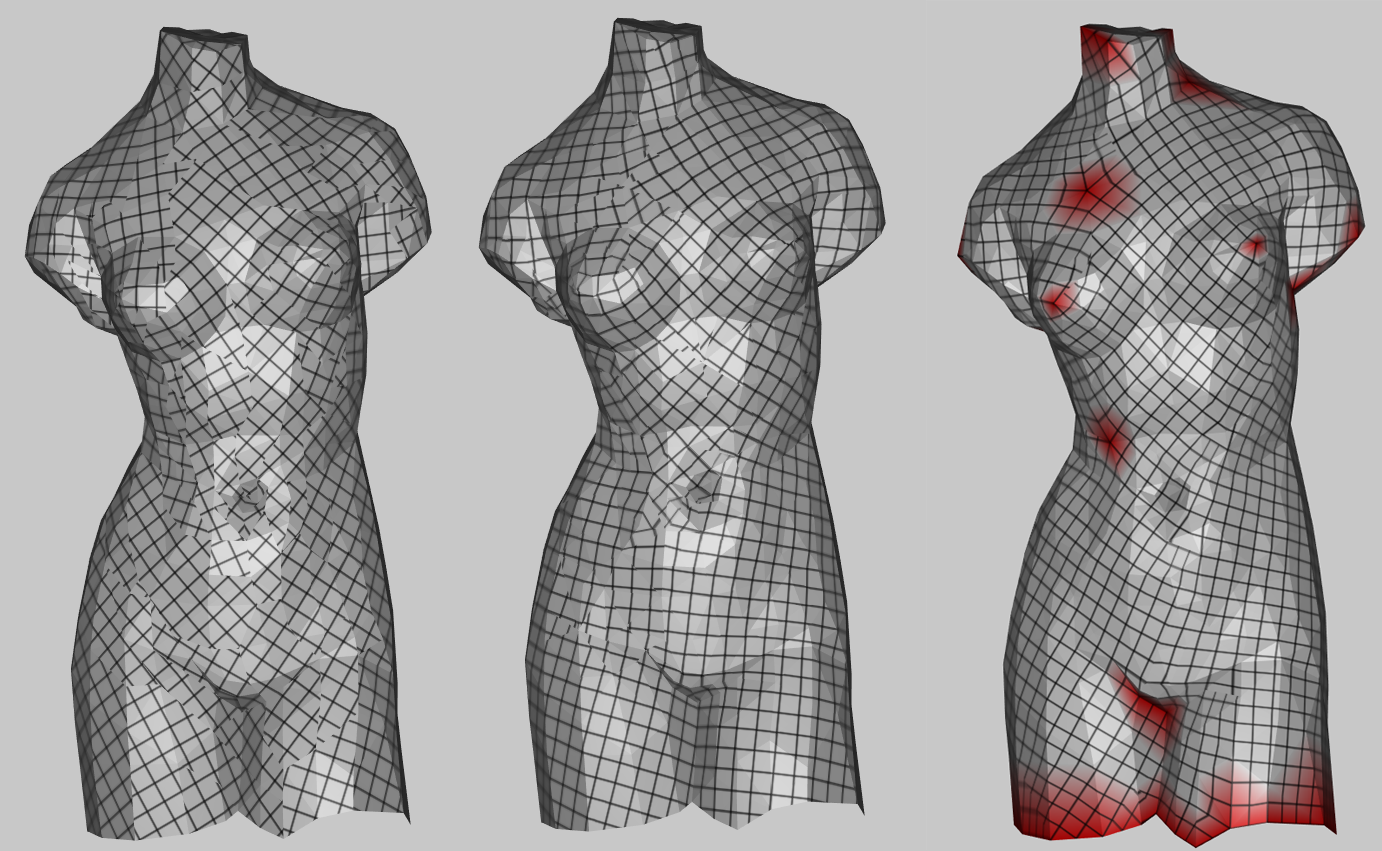
\includegraphics[width=12cm]{teaser.png}
% \selectlanguage{hebrew}
\texthebrew{\caption{\foreignlanguage{hebrew}{
\textbf{שמאל}:
תוצאת העתקת הרשת הקרטזית אל פני המשטח, לאחר המיפוי ההתחלתי של רשת המשולשים למישור
\textbf{מרכז}:
לאחר העלאת המשקולות על פונקציות המחיר
\textbf{ימין}:
התוצאה הסופית המתקבלת לאחר התכנסות תהליך האופטימיזציה למינימום מקומי המקיים את התנאים ההכרחיים והמספיקים להיווצרות רשת מרובעים ע"ג המשטח התלת מימדי
}}}
\label{fig:teaser}
\end{figure}

\selectlanguage{hebrew}
\section{הקדמה}
יישומים רבים בגרפיקה ממוחשבת, לדוגמא עיצוב דמויות ואנימציה, גיאומטריה אדריכלית, וגם סימולציה פיזית במידה מסוימת, דורשים רשת מרובעים 
\foreignlanguage{english}{Quad Mesh}
לייצוג של הגיאומטריה. עם זאת, מכיוון שמודלים מבוססי רשת משולשים
\foreignlanguage{english}{Triangle Mesh}
בדרך כלל נפוצים יותר, יש להמיר אותם באמצעות התהליך המכונה 
\foreignlanguage{english}{Quad Remeshing}.

טכניקות רבות הוצגו בשנים האחרונות, והגישה הנפוצה ביותר היא לפצל את הבעיה לייצור שדה אוריינטציה ע"ג רשת המשולשים בשלב הראשון, ומיפוי המשולשים למישור פרמטריזציה (בהנחיית השדה) בשלב השני. במסמך זה אנו מציגים גישה אינטראקטיבית ישירה וחלקה, שמבטלת את הצורך בשלבי ביניים.
הרעיון העומד מאחורי שיטות מבוססות פרמטריזציה באופן כללי, הוא למפות את רשת המשולשים המקורית למישור, וליצור עליה פריסת רשת קרטזית
\foreignlanguage{english}{Cartesian Grid}
רגילה. על מנת להבטיח שהפריסה הקרטזית במישור הופכת לרשת מרובעת תקפה על פני השטח, יש למלא תנאים מסוימים בפרמטוריזציה, המפורטים כדלהלן:

\paragraph{\foreignlanguage{english}{Seamless Condition} אי-נראות חתכים}
פונקציית המעבר
$ g_ {ij} $
בין שני חצאי קשתות
$ e_i $
ו-
$ e_j $
במישור הפרמטריזציה, המתאימים לאותה קשת המהווה חלק מחתך ע"ג רשת המשולשים המקורית, יש להיות אוטומורפיזם
\foreignlanguage{english}{Integer Grid Automorphism}
הניתן ע"י:
$$e_j = R^{r_{ij}}_{90^\circ}e_i + \vec{t}_{ij}$$
  כאשר
$r_{ij} \in \{0,1,2,3\}$ and $\vec{t}_{ij} \in \mathbb{Z}^2$.

\paragraph{\foreignlanguage{english}{Singular Points Condition} נקודות סינגולריות}
כל הקודקודים הסינגולריים, המאופיינים בפגם
זוויתי שאינו אפס במישור הפרמטריזציה, חייבים
להיות במיקומים שלמים ע"ג הרשת הקרטזית.
כלומר, בהינתן הקבוצה
$S_i$
של כל הקודקודים בתחום הפרמטריזציה, המתאימים כולם לאותו קודקוד
$v_i$
ע"ג רשת המשולשים המקורית, אנו דורשים כי:
$$\forall u \in S_i: u \in \mathbb{Z}^2 $$

\paragraph{\foreignlanguage{english}{Consistent Orientation Condition} כיוון משולשים עקבי}
כל המשולשים בתחום הפרמטריזציה צריכים להיות בעלי אוריינטציה זהה (עם כיוון-השעון או נגד כיוון-השעון). כלומר, אין לאפשר היפוך משולשים לאחר היווצרות המיפוי הראשוני.

\section{הגישה שלנו}
בהשראת \cite{Poranne:Autocuts:2017}, אנו משתמשים בגישה ישירה לבעיה של התמרת רשת משולשים לרשת מרובעים, על ידי ניסוח ופתרון של בעיית אופטימיזציה חלקה ללא אילוצים. אנו מנסחים פונקציות מחיר חלקות עבור שני התנאים הראשונים שהוזכרו לעיל (אי-נראות חתכים ונקודות סינגולריות), ומוסיפים להן פונקציית מחיר נוספת, אנרגיית דיריכלה סימטרית, המונעת היפוך משולשים ומענישה עיוות משולש.

מכיוון שכל פונקציות המחיר שלנו חלקות, אנו יכולים לבטא באופן אנליטי את הגרדיינטים ומטריצות ההסיאן שלהן, ולהשתמש בשיטת ניוטון כדי לפתור באופן איטרטיבי מיפוי שמגדיר רשת מרובעים תקפה על פני המשטח התלת-ממדי.

הגישה החלקה שלנו מאפשרת להמחיש באופן ויזואלי את כל תהליך האופטימיזציה עבור משתמש הקצה ככלי עיצוב אינטראקטיבי, המאפשר למשתמש להנחות את האלגוריתם לתוצאה הרצויה על ידי שינוי הדרגתי של משקולות העונשין, רזולוציית הרשת, הכוונה של כיוון מרובעים באמצעות מברשת כלי, ועוד. המשתמש מקבל משוב מיידי על כל שינוי שהוחל על הגדרות הבעיה. איור
1 לעיל
ממחיש את שלושת השלבים העיקריים בגישה שלנו. ראשית, משטח התלת מימד נחתך למישור. ואז, משקל פונקציית העונש החלק עלה בהדרגה. לבסוף, פונקציית העונש של נקודות בודדות מופעלת כדי להציב קודקודים בודדים במיקומים שלמים.

\section{אתחול}
אנו חותכים את רשת המשולשים על ידי מיפוי העץ הפורש הדואלי שלה למישור הפרמטריזציה באופן איזומטרי כ-"מרק משולשים"
\foreignlanguage{english}{Triangle Soup}
(פרטים נוספים על מושג זה ניתן למצוא בעבודת התזה המלאה).

ראשית אנו ממפים משולש שרירותי למישור הפרמטריזציה. לאחר מכן אנו ממפים למישור את כל המשולשים הסמוכים לו, אשר חולקים עימו קשת משותפת. אנו ממשיכים בתהליך זה אל עבר השכבה הבאה של משולשים שכנים, עד אשר כל משולשי הרשת ממופים למישור.

\section{
פונקציות מחיר
עבור אי-נראות
חתכים
\foreignlanguage{english}{(Seamless Penalty Functions)}
}

\bibliographystyle{unsrt}
\bibliography{main}

\end{document}
